\subsection{Product Perspective}
\setlength{\parskip}{1em}
\subsubsection{User scenarios}
In this section some user scenario are shown in order to explain in real life settings how the CLup application works

\textbf{Scenario 1: The Jet Market}
With the ``Stay home'' ordeal due to COVID-19 the ``Jet Market'', a mid sized grocery store in the city of Springfield saw a sudden increase of customers, but at the same time his not too big capacity was halved due to social distancing measures. These events lead to the formation of long queues of people out of the store premises in peak hours. The store manager in order to improve the service quality decided to adopt the CLup queueing system. Upon signing the contract he received a business account, and set up the shop systems with the help of CLup advisors and technicians. In the first day of CLup the queue was long as the day before, but some people seeing CLup adverts, downloaded the application. In the following days more and more people seeing that CLup allows to skip the queue by booking the visit beforehand downloaded the application. After some weeks the ``Jet Market'' can reserve up to the 60 \% of the store capacity to CLup booked customers, and the remaining is used from non CLup customer. The ``Jet Market'' manager is very happy because the queue are a lot shorter and his customer started to distribute their visit more uniformly during the day.

\textbf{Scenario 2: Bartolomeo}
Bartolomeo is an old grandfather. Due to his age he's not familiar to the modern technology, he doesn't have a smartphone. His favorite supermarket decided recently to adopt CLup, due to a long queue forming outside the store. 
Before CLup adoption Bartolomeo waited up to one hour to enter the supermarket on peak times. After the installation, for customer not confident with the modern technologies, like Bartolomeo, things did not become more complex. Bartolomeo has only to retrieve a ticket and wait until his number is called. If there are a lot of people in queue before him, he could take a sit on the bench the park near the supermarket and return in time for when his number is called, because an estimation of the entrance hour is written in the ticket.

\textbf{Scenario 3: Slightly late}
Marcello booked the 5:45 PM slot at the supermarket near his workplace. This slot allows him to enter by the 6:00 PM time slot to do some grocery shopping after work. He normally ends his workday at 5:30 PM, but his colleague asked him some help just before him leaving. He scanned the ticket at 6:05 PM, just two minutes after the 3 minute tolerance configured from the store using the CLup configuration panel. Marcello talked to the general customer assistance desk located near the gate, seeing his virtual ticket on CLup the clerk consulted the CLup operator application on his tablet and checked that the store is not totally full, the clerk scanned Marcello's ticket QR with the tablet authorizing his entrance besides his slight delay and pressed the button to open manually the gate.

\textbf{Scenario 4: Paperless}
For various reasons Adriana could not plan in advance when she can go to do grocery shopping at her favorite store. Even if she does not book her entrance in advance she use CLup to see statistics about the occupancy of the supermarket at every hour try, within her busy schedule, to avoid peak hours. When she is near the supermarket, she creates a ticket to enter as soon as possible, this ticket is equivalent to the one printed to the emitter but it's paperless. To avoid to stay in front of the entrance Adriana waits in her car until CLup notifies her that she should go to the entrance because in a short time she will enter the supermarket.

\textbf{Scenario 5: No show}
Luigi booked an entrance for the 4:00 - 4:15 PM slot. He couldn't get to the supermarket but forgot to cancel his booking even if he received some notifications before his time. At 4:20 PM the late tolerance time ended. The store at the time is unusually full and some people are waiting outside. CLup system allowed one person more to enter the store replacing Luigi that didn't come.


\subsubsection{Interfacing with external systems}
The S2B have some interfaces with some other external system used to provide data to CLup 



\textbf{Physical ticket emitter} Not all users have CLup installed in their smartphones, to allow them to enter the store a paper ticket emitter is
placed near the entrance. The ticket emitter prints tickets in 
a paper support when a button is pressed. When the button is pressed the emitter connects to internet and via a dedicated API requests a new paper ticket number. The response will contain the needed information to print the ticket and the queue statistics in the system are updated accordingly. Optionally the emitter could have a mini screen where a waiting time estimation is shown.



A \textbf{Smart gate} is a composed of a mechanical actuator that opens and closes the gate, a QR code scanner and it is provided with connectivity to internet. When a QR code is scanned and decoded, a request is sent to the CLup API containing information about the ticket scanned.
The system checks the validity of the ticket and sends a response to the gate. If the response is affirmative the gate will open, if the scanned QR doesn't represent a valid ticket an error will be shown to the customer via visual and/or auditive feedbacks. Even if the gate replaces a big part of access control staff's work (see next paragraph), some human intervention could be required for security reasons, or to open the gate in exceptional cases. 


\textbf{People counters} located at shop exits counts people passing through that exit. They are connected to the network and will communicate the count of people that left the shop. This counter could be a turnstile or a sensor or even a QR scanner that scans same tickets used to enter, or a barcode printed in the receipt. CLup system works fine without them but these counter allow to have a precise count of the people inside the shop, and this datum could be useful to estimate more precisely the waiting times.

\textbf{Ticket number screens} are located ad the shop entrance. They display the latest ticket numbers called to the entrance and the next numbers up to enter.

\subsubsection{Interfacing with users}

\textbf{Access control operators} have a portable device equipped with a camera and internet connectivity. This device has the staff access control app installed on. The operator application user interface provides these functionalities:
\begin{itemize}
    \item Authenticate with a CLup operator account or corporation SSO service
    \item Check (and adjust) estimated occupancy of the whole shop and its departments
    \item Check length of the queues, and bookings in the time slots
    \item Scan a ticket qr code to allow a person to enter
    \item Notify the next customers in the virtual ticket queue alerting them to reach the entrance
\end{itemize}

\textbf{CLup Customer Application} provides an easy to use interface with these features:
\begin{itemize}
    \item Features available to all users:
    \begin{itemize}
        \item Create a new account 
        \item Login to an existing account
        \item Show a map of nearby store adopting CLup system and an option for listing them sorted by distance
        \item See real-time and projected occupancy of all stores
    \end{itemize}
    \item Features available to authenticated users:
    \begin{itemize}
        \item Create a virtual ticket to enter in a store immediately (if space is available) or when a space is available
        \item Check store occupancy in future time slots
        \item Book a visit to a store in a time slot (if space is available) 
    \end{itemize}
\end{itemize}

\subsection{Assumptions, dependencies and constraints}
\subsubsection{Domain Assumptions}
    \begin{itemize}[label={}]
        \item DA1 Customers that created a shoplist will buy approximately all the products in that list, so they will visit for the greater part of their permanence the departments where the products are located
        \item DA2 Customer will stay approximately the time they have declared when booking the ticket
        \item DA3 The access controller works properly and won't allow unauthorized customers entrances
        \item DA4 Customers with an in-place digital ticket try to avoid to stay near the entrance until they receive the ``go to entrance notification''
        \item DA5 Customers with a booked ticket in a given time slot will not show up until few minutes before the start of their time slots
        \item DA6 If a people counter is installed it will provide the exact count of the customer that left the shop
        \item DA7 No customer are present at the shop opening hour, and no costumer will be present at the shop closing hour
        \item DA8 The store manager will insert correct data about the shop and the departments maximum capacities
    \end{itemize}
\subsubsection{Dependencies}
\subsubsection{Constraints}

\subsection{Product Functions}    
    \begin{figure}
        \centering
        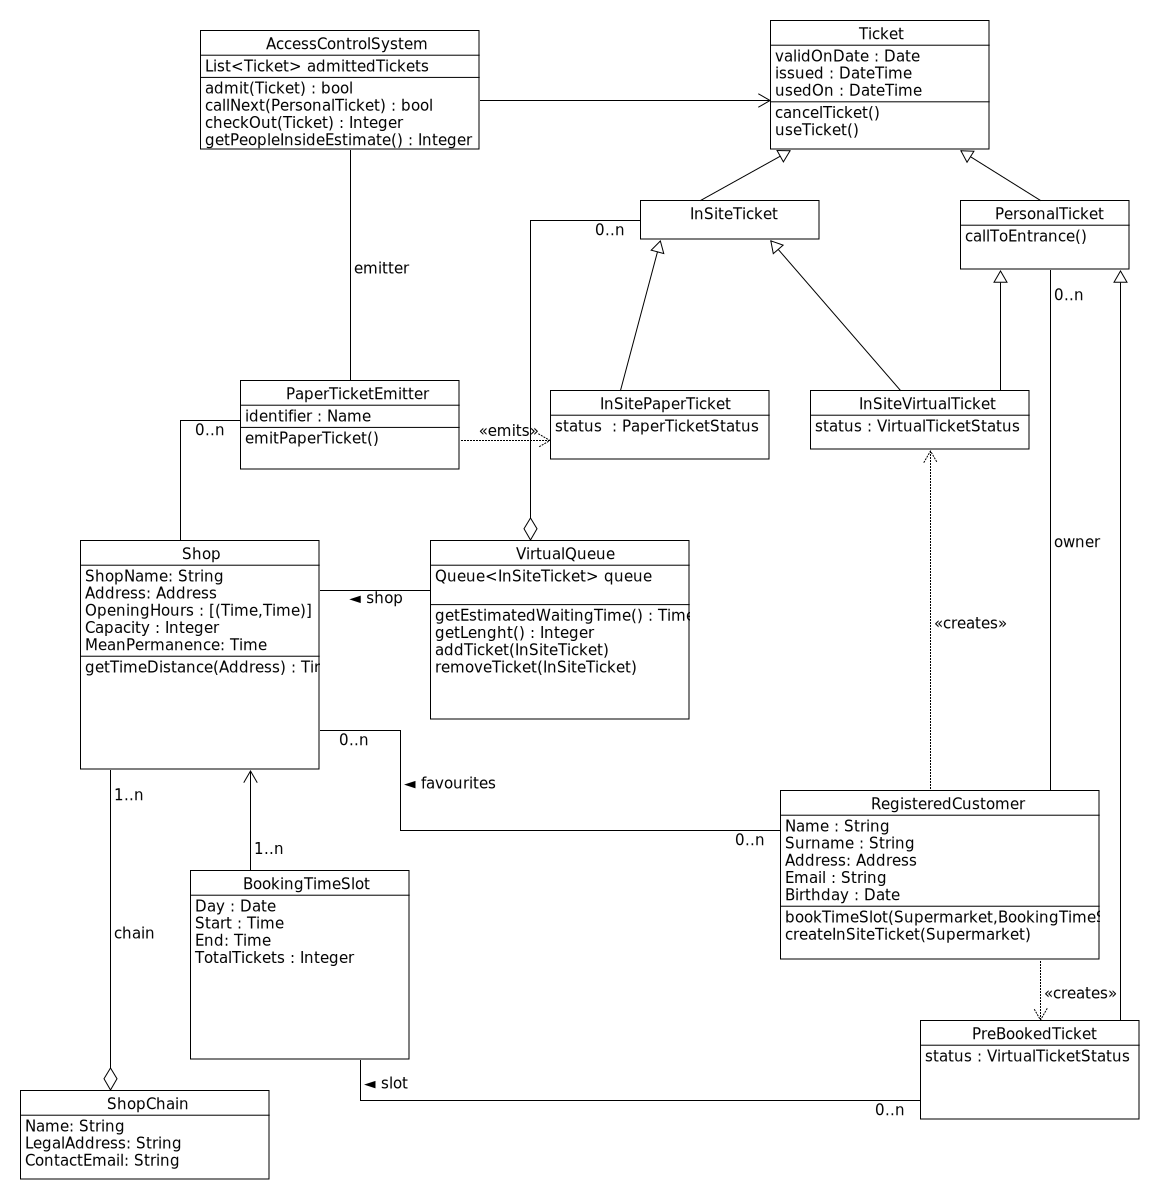
\includegraphics[width=\textwidth]{Images/UML_class_synthetic.png}
        \caption{\label{fig:Booked_Ticket_State}Class Diagram}
    \end{figure}
    \begin{figure}
    \centering
    \includegraphics[width=\textwidth]{Images/UML_booked_ticket.png}
    \caption{\label{fig:Booked_Ticket_State}Booked ticket state machine}
    \end{figure}
    The state machines depicted in the state machines below (Figures n,n+1,n+2) show the different life cycles of the three possible tickets that allow customers to enter in the supermarkets: 
    \begin{figure}
        \centering
        \includegraphics[width=\textwidth]{Images/UML_in_place_virtual_ticket.png}
        \caption{ \label{fig:Booked_Ticket_State}In place virtual ticket state machine}
    \end{figure}
    In the figure \ref{fig:Booked_Ticket_State} 
\subsection{User Characteristics}
    There are two macro-groups of people that will use CLup, the businesses adopting the system and the customers of these
    business using CLup to plan their visit to the shop.
    \subsubsection{Business-side Characteristics}
    CLup is addressed mainly to the big grocery shops, but could be used from every medium to big sized shop.
    CLup is very flexible, and will work in a lot of different scenarios, thanks to these features:
    \begin{itemize}
        \item Parameters of the system are tunable: The business could customize booking time slots duration and capacity
        \item Different access controls methods could be employed: The shop could install some smart gates with a QR scanner
              or could hire an employee that checks the tickets with a mobile device using the business CLup application. 
        \item Different precision levels of estimated data are possible, based on the data sources available:
              For example if the shop counts the number of people exiting the premises (using a turnstile or a QR scanner) 
              CLup will provide the exact occupancy, but if this is not possible an estimation will be provided, based on the 
              average permanence time in the shop.  
          
    \end{itemize}
    \subsubsection{Customer side characteristics}
    All the people need to do grocery shopping especially during the lockdown measures enacted due to COVID-19. 
    Every one should be able to access the shop, even the people that can't download the CLup application.
    The S2B solves this problem by allowing the customer a paper ticket and wait in a physical line before entering the shop if the shop is full.
    The physical line of customer is unavoidable if the supermarket could not satisfy the increased demand of groceries in its catching area, even if CLup could alleviate this problem allowing to better distribute the customer visits during the shop opening hours. The possibility of booking the visit in advance will push more and more users to download CLup to avoid the queue, and be safer avoiding to cram at the entrance.


